\documentclass[16pt]{beamer}
\usepackage[utf8]{inputenc}
\usepackage[croatian]{babel}
\usepackage{graphicx}
\usepackage{verbatim}
\usepackage{graphicx}
\graphicspath{ {figures/} }
\usepackage{array}
\usetheme{Warsaw}
\definecolor{mygreen}{rgb}{0.3, 0.73, 0.09}
\setbeamercolor*{palette primary}{use=structure,fg=black,bg=mygreen}
\definecolor{mygreen1}{rgb}{0.0, 0.5, 0.0}
\setbeamercolor*{palette quaternary}{fg=black,bg=mygreen1}

\title[IZRADA TABLICA I GRAFIKONA\hspace{20mm} \insertframenumber/\inserttotalframenumber]{IZRADA TABLICA I GRAFIKONA}
\author{Anamaria Vargić \  Jelena Stojković  \  Valentina Ecimović}
\institute{Tehnički fakultet u Rijeci - Računarstvo}
\date{2018}
 
\begin{document}
\frame{\titlepage}
%slajd sa sadrzajem
\begin{frame}

\frametitle{Sadržaj}

\tableofcontents

\end{frame}
\begin{frame}
\frametitle{Lista tabela i slika}
	\listoffigures
 	\listoftables
 	\newpage
 	\pagenumbering{arabic}
\end{frame} 

\begin{frame}
\frametitle{Izdrada tablica iz .csv datoteka} 
    \begin{itemize}    	
        \item .csv (comma separated value) datoteke možemo proizvesti u programima kao što su Microsoft Excel i Google spreadsheet
        \item stvaranje tablica iz .csv datoteka nam omogućava \textbf{pgfplotstable} paket
        \item potrebno je učitati paket u preambulu dokumenta
        \item ovu metodu generiranja tablica koristimo kada radimo s velikim količinama podataka	
    \end{itemize}   
\end{frame}

\begin{frame}
\frametitle{primjer tablice}
	\begin{figure}
		\includegraphics[width=0.8\linewidth]{tablica.png}
		\caption{Tablica 1}
	\end{figure}
\end{frame}

\begin{frame}[fragile]
\frametitle{primjer tablice}
\begin{verbatim}
\begin{document}
\pgfplotstabletypeset[
col sep = comma,
string replace*={_}{\textsubscript},
every head row/.style={before row=\toprule,after row=\midrule},
every last row/.style={after row=\bottomrule},
display columns/0/.style={string type,column name={}}
]
{avg_value.csv} %ovdje ide naziv vase .csv datoteke

\end{document}
\end{verbatim}
\end{frame}

\begin{frame}[fragile]
\frametitle{Konturni grafikoni}
	\begin{itemize}
		\item koristeći \textbf{pgfplots} paket možemo stvarati i konturne grafikone	
	\end{itemize}	
	\begin{figure}
		\includegraphics[width=1.5\linewidth]{konturni.png}
		\caption{Konturni graf}
	\end{figure}
\end{frame}

\begin{frame}[fragile]
\frametitle{Konturni grafikoni}
	\begin{verbatim}
\begin{document}

\begin{tikzpicture}
\begin{axis}
[
    title={},
    view={0}{50}
]
\addplot3[
    contour gnuplot={levels={0.9, 0.5, 0.2, -0.3}}
]
{sin(deg(sqrt(x^2+y^2)))/sqrt(x^2+y^2)};
\end{axis}
\end{tikzpicture}

\end{document}
	\end{verbatim}
\end{frame}

\begin{frame}[fragile]
\frametitle{Konturni grafikoni}
	\begin{verbatim}
		view={0}{50}
	\end{verbatim}
	\begin{itemize}
		\item mijenjanjem vrijednosti u zagradama se rotiramo oko z osi odnosno x osi
	\end{itemize}
	\begin{verbatim}
		 contour gnuplot={levels={0.9, 0.5, 0.2, -0.3}}
	\end{verbatim}
	\begin{itemize}
		\item koristimo vanjski softver gnuplot za računanje konturnih linija
		\item parammetar levels diktira na kojim će se vrijednostima graf izdizati tj. gdje će se pojavljivati konturne linije
	\end{itemize}	
\end{frame}

\begin{frame}
\frametitle{Grafikon površine}
	\begin{figure}
		\includegraphics[width=1.5\linewidth]{povrsina.png}
		\caption{Grafikon površine}
	\end{figure}
\end{frame}

\begin{frame}[fragile]
\frametitle{Grafikon površine}
	\begin{verbatim}		
\begin{document}

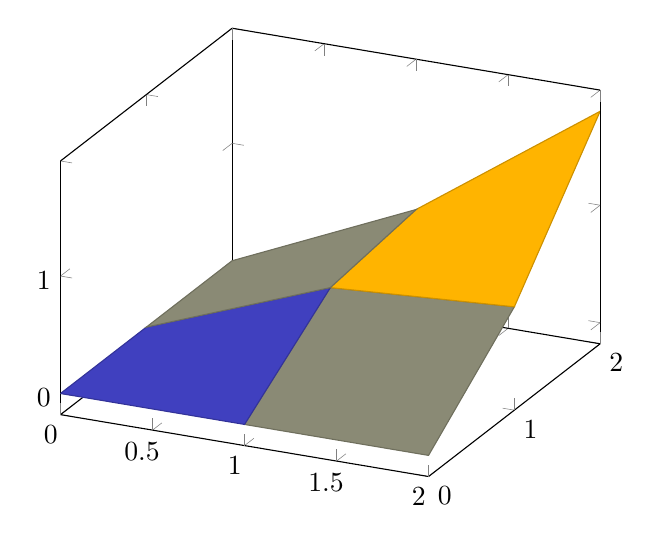
\begin{tikzpicture}
\begin{axis}
\addplot3[
    surf,
] 
coordinates {
(0,0,0) (0,1,0) (0,2,0)

(1,0,0) (1,1,0.6) (1,2,0.7)

(2,0,0) (2,1,0.7) (2,2,1.8)
};
\end{axis}
\end{tikzpicture}
\end{document}
	\end{verbatim}
\end{frame}

\begin{frame}
\frametitle{Grafikon površine}
	\begin{itemize}
		\item unošenjem koordinata točaka u obliku matrice dobit ćemo grafikon površine
		\item naredbe za oblikovanje 3D grafikona vrijede i za oblikovanje ovog grafikona
	\end{itemize}	
\end{frame}


\end{document}


 
 
